\documentclass[12pt,a4paper]{article}

\usepackage[utf8]{inputenc}
\usepackage[T1]{fontenc}
\usepackage[polish]{babel}
\usepackage{geometry}
\usepackage{graphicx}
\usepackage{float}
\usepackage{hyperref}
\usepackage{amsmath}
\usepackage{booktabs} % Dodane dla \toprule, \midrule, \bottomrule

\geometry{margin=2.5cm}

\title{Projekt 12: Ocena ryzyka deszczu i krótkoterminowa predykcja}
\author{Kornel Wasilewski\\Maciej Truchanowski}
\date{}

\begin{document}

\maketitle

\section{Cel projektu}

Celem projektu jest oszacowanie krótkoterminowego ryzyka deszczu na podstawie ostatnich pomiarów pogodowych pobranych ze współdzielonego Weather REST API. System przetwarza dane pogodowe, tworzy cechy kroczące, oblicza wynik ryzyka deszczu w skali od 0 do 100 oraz przewiduje, czy deszcz wystąpi w kolejnym pomiarze.

Projekt skupia się na pełnym potoku przetwarzania danych. Obejmuje pobranie danych z API, zapisanie danych surowych, czyszczenie danych, tworzenie cech, obliczenie wyniku analitycznego, ewaluację oraz wizualizację rezultatów.

\section{Źródło danych}

Głównym źródłem danych jest współdzielone Weather REST API. Projekt korzysta z endpointu batch, który pobiera ostatnie pomiary pogodowe dla stacji GDN 01.

\begin{itemize}
\item Base URL: \url{https://e6uw49pbah.execute-api.us-east-1.amazonaws.com/dev}
\item Endpoint: batch weather endpoint dla stacji GDN 01 z limitem 100 pomiarów
\item Metoda autoryzacji: Bearer token
\end{itemize}

Odpowiedź API zawiera pomiary pogodowe z następującymi polami:

\begin{itemize}
\item timestamp,
\item station id,
\item temperature,
\item humidity,
\item pressure,
\item wind speed,
\item wind direction,
\item rain amount,
\item cloud cover.
\end{itemize}

\section{Architektura systemu}

Zaimplementowana architektura odpowiada typowemu potokowi przetwarzania danych:

\begin{center}
Weather REST API $\rightarrow$ dane surowe $\rightarrow$ czyszczenie danych $\rightarrow$ tworzenie cech $\rightarrow$ scoring $\rightarrow$ ewaluacja $\rightarrow$ wykresy
\end{center}

Projekt został podzielony na osobne moduły Pythona:

\begin{itemize}
\item ingest.py -- pobiera dane pogodowe z REST API i zapisuje surowe dane w formacie JSON.
\item process.py -- wczytuje dane surowe, sprawdza kolumny, czyści rekordy, usuwa duplikaty i zapisuje czysty zbiór danych.
\item features.py -- tworzy cechy kroczące i opóźnione wykorzystywane w analizie ryzyka deszczu.
\item scoring.py -- oblicza wynik ryzyka deszczu i przypisuje klasy ryzyka.
\item evaluate.py -- ocenia wyniki predykcji za pomocą metryk klasyfikacyjnych i generuje wykresy.
\item main.py -- uruchamia cały potok od pobrania danych do ewaluacji.
\end{itemize}

\section{Struktura przechowywania danych}

Projekt wykorzystuje lokalną strukturę plików podzieloną na warstwę danych surowych, przetworzonych i wynikowych.

\begin{verbatim}
data/
|-- raw/
|   |-- weather_raw.json
|
|-- processed/
|   |-- weather_clean.csv
|   |-- weather_features.csv
|
|-- output/
|   |-- rain_risk_scored.csv
|   |-- evaluation_metrics.txt
|   |-- rain_risk_chart.png
|   |-- confusion_matrix.png
\end{verbatim}

Taka struktura oddziela dane surowe pobrane z API od danych wyczyszczonych, cech analitycznych oraz końcowych wyników projektu.

\section{Czyszczenie danych}

Etap czyszczenia danych przekształca surową odpowiedź API w uporządkowany zbiór tabelaryczny. Wykonywane są następujące operacje:

\begin{itemize}
\item parsowanie znaczników czasu do formatu daty i czasu,
\item konwersja kolumn liczbowych do typów numerycznych,
\item usunięcie rekordów bez znacznika czasu lub identyfikatora stacji,
\item usunięcie duplikatów,
\item sortowanie rekordów według stacji i czasu,
\item ograniczenie wartości wilgotności i zachmurzenia do zakresu 0--100,
\item zabezpieczenie przed ujemnymi wartościami opadu i prędkości wiatru.
\end{itemize}

Po czyszczeniu zbiór danych zawierał 100 rekordów.

\section{Tworzenie cech}

Tworzenie cech polega na przygotowaniu dodatkowych zmiennych na podstawie ostatnich pomiarów pogodowych. Cechy te opisują krótkoterminowe trendy pogodowe i są używane jako wejście do modelu oceny ryzyka deszczu.

W projekcie utworzono następujące cechy:

\begin{table}[H]
\centering
\begin{tabular}{p{5.5cm} p{8.5cm}}
\toprule
\textbf{Cecha} & \textbf{Opis} \\
\midrule
Średnia krocząca wilgotności & Średnia wilgotność z 3 ostatnich pomiarów. \\
Średnia krocząca zachmurzenia & Średnie zachmurzenie z 3 ostatnich pomiarów. \\
Średnia krocząca prędkości wiatru & Średnia prędkość wiatru z 3 ostatnich pomiarów. \\
Suma niedawnych opadów & Suma opadów z 3 ostatnich pomiarów. \\
Zmiana ciśnienia & Różnica między bieżącą a poprzednią wartością ciśnienia. \\
Poprzedni opad & Wielkość opadu z poprzedniego pomiaru. \\
Czy spadnie deszcz & Binarna zmienna docelowa wskazująca, czy w następnym pomiarze wystąpi opad deszczu. \\
\bottomrule
\end{tabular}
\caption{Wygenerowane cechy}
\end{table}

Po etapie tworzenia cech zbiór danych zawierał 98 rekordów, ponieważ część rekordów nie mogła zostać użyta do cech opóźnionych i predykcji kolejnego pomiaru.

\section{Metody analityczne}

W projekcie wykorzystano trzy główne metody analityczne: klasyfikację binarną, regułowy model bazowy oraz ewaluację za pomocą precision i recall.

\subsection{Klasyfikacja binarna}

Zadanie predykcyjne zostało sformułowane jako problem klasyfikacji binarnej. Zmienna docelowa ma dwie możliwe wartości:

\begin{itemize}
\item 0 -- deszcz nie wystąpi w kolejnym pomiarze,
\item 1 -- deszcz wystąpi w kolejnym pomiarze.
\end{itemize}

Zmienna binarna jest tworzona poprzez sprawdzenie, czy deszcz występuje w kolejnym pomiarze. Dzięki temu projekt realizuje krótkoterminową predykcję deszczu.

\subsection{Regułowy model bazowy}

Regułowy model bazowy oblicza wynik ryzyka deszczu w skali od 0 do 100. Wynik opiera się na zmiennych pogodowych, które są logicznie powiązane z ryzykiem deszczu: wilgotności, zachmurzeniu, spadku ciśnienia, poprzednim opadzie i prędkości wiatru.

Wagi wykorzystane w systemie scoringowym są następujące:

\begin{table}[H]
\centering
\begin{tabular}{p{6cm} p{4cm}}
\toprule
\textbf{Zmienna} & \textbf{Waga} \\
\midrule
Wilgotność & 30 procent \\
Zachmurzenie & 25 procent \\
Spadek ciśnienia & 20 procent \\
Poprzedni opad & 15 procent \\
Prędkość wiatru & 10 procent \\
\bottomrule
\end{tabular}
\caption{Wagi wskaźnika ryzyka opadów}
\end{table}

Końcowy wynik ryzyka deszczu jest liczony według wzoru:

\[
R = 0.30H + 0.25C + 0.20P + 0.15D + 0.10W
\]

gdzie:

\begin{itemize}
\item R oznacza końcowy wynik ryzyka deszczu,
\item H oznacza wynik wilgotności,
\item C oznacza wynik zachmurzenia,
\item P oznacza wynik spadku ciśnienia,
\item D oznacza wynik poprzedniego opadu,
\item W oznacza wynik prędkości wiatru.
\end{itemize}

Następnie wynik jest przekształcany na klasę ryzyka:

\begin{itemize}
\item 0--33: niskie ryzyko,
\item 34--66: średnie ryzyko,
\item 67--100: wysokie ryzyko.
\end{itemize}

System przewiduje deszcz, gdy wynik ryzyka deszczu jest większy lub równy 60.

\subsection{Ewaluacja precision i recall}

Jakość predykcji została oceniona za pomocą standardowych metryk klasyfikacyjnych:

\begin{itemize}
\item accuracy,
\item precision,
\item recall,
\item F1-score,
\item macierz pomyłek.
\end{itemize}

Precision określa, jak często system miał rację, gdy przewidział deszcz. Recall określa, jak wiele rzeczywistych przypadków deszczu zostało wykrytych przez system.

\section{Wyniki}

Potok przetwarzania został uruchomiony poprawnie. Program pobrał dane pogodowe, przetworzył zbiór danych, obliczył wyniki ryzyka deszczu, wygenerował predykcje oraz ocenił rezultaty.

Uzyskane metryki ewaluacyjne były następujące:

\begin{table}[H]
\centering
\begin{tabular}{lc}
\toprule
\textbf{Metryka} & \textbf{Wartość} \\
\midrule
Accuracy & 0.3571 \\
Precision & 0.5833 \\
Recall & 0.2090 \\
F1-score & 0.3077 \\
\bottomrule
\end{tabular}
\caption{Metryki ewaluacyjne}
\end{table}

Wartość precision równa 0.5833 oznacza, że gdy system przewidywał deszcz, miał rację w około 58 procentach przypadków. Wartość recall równa 0.2090 oznacza, że system wykrył około 21 procent wszystkich rzeczywistych przypadków deszczu.

Oznacza to, że model regułowy jest dość konserwatywny. Nie przewiduje deszczu bardzo często, ale gdy już to robi, jego predykcja jest poprawna w ponad połowie przypadków.

\section{Wykresy}

Projekt generuje dwa wyniki wizualne: wykres wyniku ryzyka deszczu w czasie oraz macierz pomyłek dla klasyfikacji binarnej.

\subsection{Wynik ryzyka deszczu w czasie}

Pierwszy wykres przedstawia wynik ryzyka deszczu w czasie. Zawiera również próg predykcji równy 60.

\begin{figure}[H]
\centering
\IfFileExists{data/output/rain_risk_chart.png}{
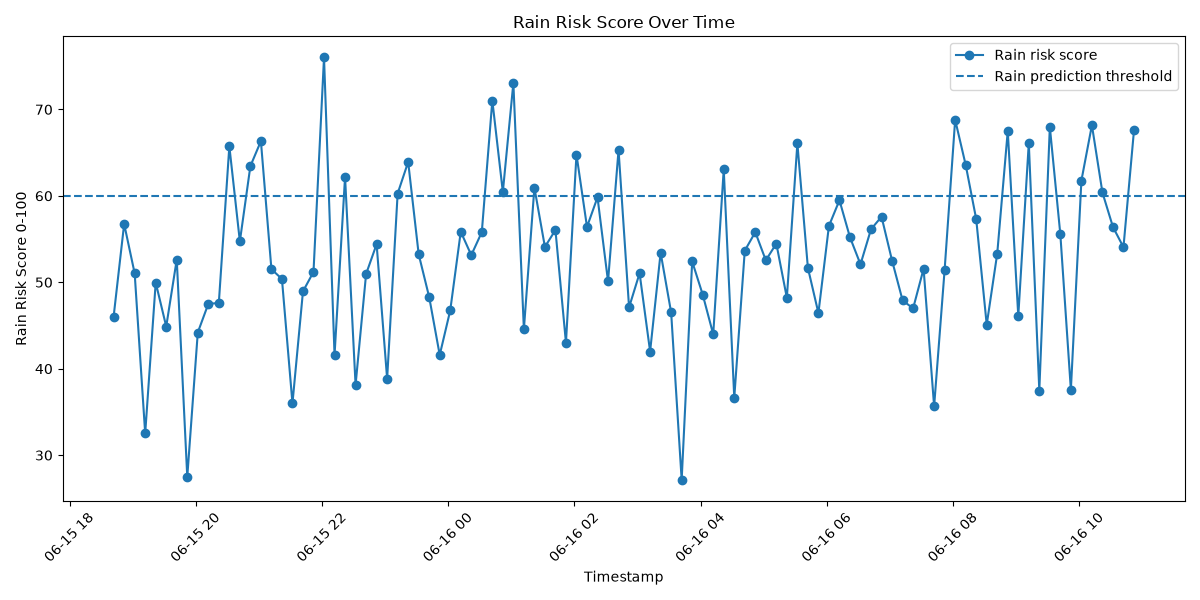
\includegraphics[width=0.95\textwidth]{data/output/rain_risk_chart.png}
}{
\fbox{\parbox{0.9\textwidth}{Nie znaleziono pliku z wykresem ryzyka deszczu. Należy wgrać wygenerowany wykres do Overleaf albo zmienić ścieżkę do obrazka.}}
}
\caption{Wynik ryzyka deszczu w czasie}
\end{figure}

\subsection{Macierz pomyłek}

Drugi wykres przedstawia macierz pomyłek dla binarnej predykcji deszczu.

\begin{figure}[H]
\centering
\IfFileExists{data/output/confusion_matrix.png}{
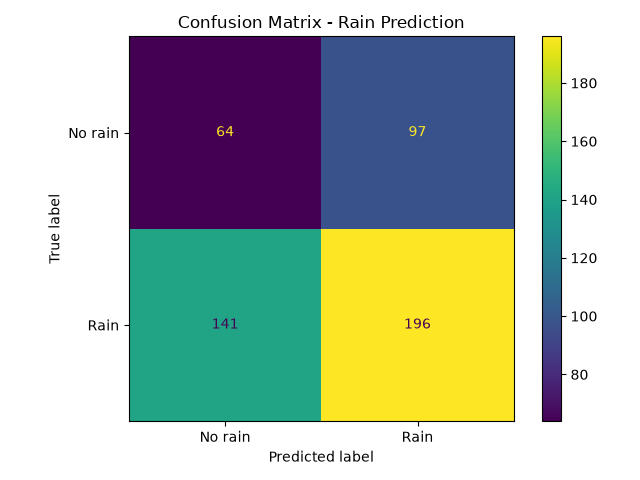
\includegraphics[width=0.75\textwidth]{data/output/confusion_matrix.png}
}{
\fbox{\parbox{0.9\textwidth}{Nie znaleziono pliku z macierzą pomyłek. Należy wgrać wygenerowany wykres do Overleaf albo zmienić ścieżkę do obrazka.}}
}
\caption{Macierz pomyłek dla predykcji deszczu}
\end{figure}

\section{Wnioski}

Projekt poprawnie implementuje pełny potok przetwarzania danych dla krótkoterminowej predykcji ryzyka deszczu. System pobiera dane z REST API, zapisuje surową odpowiedź, czyści zbiór danych, tworzy cechy kroczące, oblicza regułowy wynik ryzyka deszczu oraz ocenia jakość predykcji.

Zaimplementowany model osiągnął precision na poziomie 0.5833 oraz recall na poziomie 0.2090. Oznacza to, że model lepiej radzi sobie z unikaniem fałszywych predykcji deszczu niż z wykrywaniem wszystkich rzeczywistych przypadków deszczu. Stosunkowo niska wartość recall pokazuje, że wiele rzeczywistych przypadków opadu nie zostało wykrytych.

\end{document}
